\documentclass[11pt, oneside]{article} 	% use "amsart" instead of "article" for AMSLaTeX format
\usepackage{geometry} 		% See geometry.pdf to learn the layout options. There are lots.
\geometry{letterpaper}  		% ... or a4paper or a5paper or ... 
\usepackage[parfill]{parskip} 		% Activate to begin paragraphs with an empty line rather than an indent
\usepackage{graphicx}				% Use pdf, png, jpg, or eps§ with pdflatex; use eps in DVI mode
								% TeX will automatically convert eps --> pdf in pdflatex		
\usepackage{amssymb}
\usepackage{amsmath}
\usepackage{authblk}
\usepackage[
backend=biber,
style=alphabetic,
]{biblatex}
\usepackage{graphicx}
\graphicspath{ {./images/} }
\usepackage{verbatim}
\usepackage{tikz} 
\tikzset{
    vertex/.style={circle,draw,minimum size=1.5em},
    edge/.style={->,> = latex'}
}
\usetikzlibrary{arrows}
\usepackage{subcaption}
\usepackage{hyperref}
\usepackage{xcolor,colortbl}

\usepackage{listings}
\lstset{
basicstyle=\small\ttfamily,
columns=flexible,
breaklines=true
}
\usepackage{syntonly}
% \syntaxonly <-- use this for checking syntax only
% \mbox {text} - keep together
% \fbox {text} - keep together and draw around

%\pagestyle{plain|headings|empty} % header and footer p.27
%SetFonts
%\include{filename}, \includeonly{filename1, filename2} , \input[fiename}

%SetFonts% 

\title{Strategy for bitches (a dice game)}
\author{Dave Fetterman}
\affil{Obviously Unemployed}
\date{8/14/22}
\begin{document}
\maketitle

\begin{abstract}

This paper details a decision framework for playing well at bitches (a dice game), introduced to me by Larry Waldman.  Mr. Waldman asked for a truly \emph{optimal} strategy but, like blackjack, the state of the game is too large for a human to remember during gameplay.  With some simplifications, we can produce a memorizable ``blackjack table'' that performs reasonably well.

\end{abstract}

\section{Introduction}

Following is a series of desperately important text messages from Larry ``F.'' Waldman about the game ``bitches (a dice game)'', buyable here (\url{https://gluebunnygames.com/products/bitches-a-dice-game}), or easy to assemble from fifteen dice and the frantic instructions below in Figs.~\ref{fig:larry1} and ~\ref{fig:larry2}.

\begin{figure}[!htb]
\begin{lstlisting}
Gotta tell you about this game. I need a paper on the game theory optimized strategy
\end{lstlisting}
\caption{Larry has to talk to me}
\label{fig:larry1}
\end{figure}


\begin{figure}[!htb]
\begin{lstlisting}
12 regular dice + 1 8 sided die, 1 10 sided die, 1 12 sided die. 

Roll all the dice. You must take at least one die out each roll. If the die (or dice) you remove are not their max value (eg 6 for a regular die), you get max - <die value> amount of points. So for example if you take away a regular die showing four, you get two points. 

Points are bad. 

After all the dice are gone, add up your points and that is your score.
\end{lstlisting}
\caption{Larry is unhelpful after this point}
\label{fig:larry2}
\end{figure}

I find the use of ``regular dice'' to be six-normative but agree to proceed with the following two missions:
\begin{itemize}
\item Determine the strategy for getting the best expected score (``optimal strategy'').
\item Determine the expected number of points from playing that strategy.
\end{itemize}

\emph{Note: I generally proceed with solving an equivalent game: picking up a die gives you as many points as the face value}.  So, instead of getting one (bad) point when picking up a six-sided die showing five, you receive five (good) points.  A score minimizing strategy using the ``bitches'' scoring system and one maximizing this scoring system are equivalent; accepting a die with $s$ sides gives you $s-p$ (bad) points in the first system and $p$ in the second.  We can convert ``expected face value'' to ``expected `b (a. d. g.)' points'' trivially when we're done.


The proof/algorithm sketch:
\begin{itemize}
\item Section~\ref{section:solve-one}: We can solve the game definitively for one die of any size.
\item Section~\ref{section:solve-perfect}: Solving the game perfectly for the standard ``bitches'' setup (15 dice of sizes indicated in Fig.~\ref{fig:larry2}) requires evaluating way too many states and transitions to be feasible, fun, or useful in play.
\item Section~\ref{section:split-out}: We propose a simple strategy: We can reduce the game by considering 15 dice as each playing parallel and separate single-die games and bear the cost when this ends up being untrue.  We calculate a guess at a ``typical'' score with this strategy.
\item Section~\ref{section:simultation}: We use computers to validate.
\end{itemize}

\section{Solving the one die case} \label{section:solve-one}

As the old saying goes, ``if you cannot play chess well with 3 pieces, you cannot play well with 32.''  Therefore, in chess, we study endgames first and here, first solve the game with played with a single die with unique incremental pip counts $1, 2, 3 ... s$ up to some arbitrary $s$.

Though we make a misstep in solving this next (the Aside section), the following principle is rock solid.

\fbox{\parbox{\textwidth}{
\textbf{Principle: Know when to quit}
\begin{itemize}
\item We establish an optimal strategy for the base case $r = 1$ (one roll remaining).
\item With $r > 1$ rolls remaining, if accepting the current value of the die has a higher expected value than the expected value using the optimal strategy going forward, accept the die value.  Else roll.
\end{itemize}
}}

If\footnote{We do: we only have the option of accepting the roll.  Expected face value is clearly $\frac{s+1}{2}$.} we have an optimal strategy for $r=1$, then we necessarily have one for $r=2, 3... $ and so on.

\subsection{Aside: (Incorrectly) using the expected maximum future roll}

We will now take a misstep in finding the optimal strategy, an example of an intuitive but wrong move in probabilistic thinking.  It helps illustrate why the best strategy is best, and so we include it.

The logic: We, of course, want to choose the best future roll from this die, so the \textbf{expected max strategy} is \emph{if the current roll is worse than the expected future maximum among the $r$ rolls remaining, keep rolling. Otherwise, pick up the die and accept the points}.

This \emph{seems} like the right idea.  After all, if we can expect our future rolls to include a better roll on average, we should keep rolling, right?  This is true, but not the whole story.  

At least it's easy to calculate.  Given $s$ (a singe die's number of sides) and $r$ rolls remaining, the expected value of the max roll value $m$ is straightforward:
\begin{align}
p_{m \leq k}(r) =  (\frac{k}{s})^r \\
p_{m \leq k-1}(r) =  (\frac{k-1}{s})^r \\
p_{m = k}(r) =  (\frac{k}{s})^r - (\frac{k-1}{s})^r \\
E_r = \sum_{k=1}^s k[\frac{k^r - (k-1)^r}{s}]
\end{align}

For any given number of pips $k$ between 1and $s$:
\begin{itemize}
\item (1) is the probability that all of the $r$ rolls are between 1 and $k$.
\item (2) is the probability that all of the $r$ rolls are between 1 and $k-1$.
\item (3) subtracts these two for the probability that the max roll is exactly $k$ (as in, there's at least one $k$ roll in the space of (1)).
\item (4) is the familiar expected value formula.
\end{itemize}

 Fig.~\ref{fig:max-rolls}.shows the results for 6-, 8-, 10-, and 12-sided dice.

\begin{figure}[!htb]
\centering
\begin{tabular}{c | c c c c}
$r$ & $s=6$ & $s=8$  & $s=10$ & $s=12$  \\
\hline
1 & 3.5 & 4.5 & 5.5 & 6.5 \\
2 & 4.472 & 5.812 & 7.15 & 8.486 \\
3 & 4.958 & 6.469 & 7.975 & 9.479 \\
4 & 5.245 & 6.858 & 8.467 & 10.072 \\
5 & 5.431 & 7.115 & 8.792 & 10.465 \\
6 & 5.56 & 7.295 & 9.022 & 10.744 \\
7 & 5.654 & 7.428 & 9.192 & 10.952 \\
8 & 5.724 & 7.529 & 9.323 & 11.111 \\
9 & 5.778 & 7.608 & 9.426 & 11.238 \\
10 & 5.82 & 7.67 & 9.509 & 11.34 \\
11 & 5.853 & 7.721 & 9.576 & 11.424 \\
12 & 5.88 & 7.763 & 9.633 & 11.495 \\
13 & 5.901 & 7.798 & 9.68 & 11.554 \\
14 & 5.919 & 7.827 & 9.72 & 11.605 \\
15 & 5.933 & 7.851 & 9.754 & 11.648 \\
\end{tabular}
\caption{Expected max roll of an $s$-sided die over $r$ rolls}
\label{fig:max-rolls}
\end{figure}

We then, look to the expected value of the next state and pick up our die if the value equals or exceeds our expected future value.  For example, if we're rolling a 6-sided die and we have three rolls left, after rolling we pick up if and only if the roll exceeds what we'd expect by taking our shot with two rolls left (4.472).  This means we'd pick up a 5 or 6.  If we continue, we would pick up anything equal to or exceeding 3.5 ($r=1, s=6$).

\subsection{Why doesn't this work?}

Though we would like to choose the maximum roll across our future rolls, and we can be reasonably confident some high numbers are ahead of us if we have many rolls remaining, we have a problem: \emph{we are not guaranteed to choose the max roll when we see it}, even when appropriarly we adjust our expectations of the max roll \emph{down} as we near the end of the cliff as in Fig.~\ref{fig:max-rolls}.

\textbf{Counterexample to max strategy}

Consider this example with a 50-sided die and three rolls remaining, with $E_{max}(s, r)$ signifying the expected value of the \textbf{max} roll over $r$ rolls of a $s$-sided die, which can be computed with formula (4) above.

\begin{itemize}
\item $E_{max}(50, 1) = 25.5$.  You must pick up once rolled.
\item $E_{max}(50,2) = 33.83$.  You should pick up if your roll equals or exceeds $\lfloor E_{max}(50, 1)\rfloor = 25$.
\item $E_{max}(50,3) = 37.995$.  You should pick up if your roll equals or exceeds $\lfloor E_{max}(50,2) \rfloor = 33$.
\end{itemize}
 

\begin{comment}
 \textbf{best strategy}
\begin{itemize}
\item 25.5 - no cutoff
\item 31.75 - cutoff 25
\item 35.625 - cutoff 31
\end{itemize}
\end{comment}

The reroll cutoff (inclusive) on $r=2$ will be 25 for any optimal strategy, since no decisions are possible for $r=1$.   The EV is 31.75.

\begin{align}
E(2)  = \sum_{k=26}^{50} \frac{k}{50} + \frac{25}{50}*25.5 = 31.75 \\
\end{align}

So we look at the expected value of five strategies (A, B(est), C, M(ax), D) then, which are exactly the different cutoffs when $r=3$: (31, 32, 33, 34, 35), respectively:

\begin{align}
E_A(3) = \sum_{k=31}^{50} \frac{k}{50} + \frac{30}{50} (31.75) = 35.25 \\
E_B(3) = \sum_{k=32}^{50} \frac{k}{50} + \frac{\textbf{31}}{50} (31.75) = \textbf{35.265} \\
E_C(3) =  \sum_{k=33}^{50} \frac{k}{50} + \frac{32}{50} (31.75) = 35.260 \\
E_M(3) = \sum_{k=34}^{50} \frac{k}{50} + \frac{\textbf{33}}{50}(31.75) = 35.235 \\
E_D(3) = \sum_{k=35}^{50} \frac{k}{50} + \frac{34}{50} (31.75) = 35.19 \\
\end{align}

We see that the expected value of our strategy peaks not at our supposed max strategy of rerolling at 33 or less, but rerolling at 31 or less (accepting 32 and 33).

This counterexample proves that max is not the optimal strategy, though not by a whole lot for this small (and easily calculable) example.  The real intuition comes from considering that, for example, if we're three rolls out on a 50-sider, there is a \emph{possibility} that there are one or even \emph{two} fifties in my future; those will drive up the expected maximum roll.  However, the likelihood that I will encounter them is diminished by the change that I'm rolling high thirties or above before that. 

Three future in-order rolls of (35, 1, 50) and (50, 1, 35) both contribute 50 equally to the expected maximum.  However, I will never encounter the first case, since I will have optimally picked up the 35 by then, which `shadows' the high rolls.  Note that (35, 1, 10) doesn't `shadow' a future low roll, since the maximum is not the third number but 35.

If this isn't intuitive enough, consider that on a 1000-sided die with three rolls left, you have to exclude the possibility of the sequence (999, *, 1000).  This part of the possibility space contributes 1000 to the max strategy, but to no reasonable strategy otherwise.  This is why our EVs for the optimal strategy will be lower than the intuitive ``pick the expected future maximum''.  Instead, we need to ``pick the expected future maximum \emph{that we will select}''.

\subsection{Solving the one-die case optimally}

Though there doesn't appear to be a closed form for the expectations and cutoffs of the optimal strategy, determining it is no big shakes.  If we have $r$ rolls left for a die of size $s$, and we have the optimal expected value $E(r-1, s)$ for the version of the problem with one less roll, our optimal strategy, according to the \emph{Know when to quit principle}, is to keep rolling unless we equal or exceed the value of continuing.  For ease of reading, we introduce cutoff $c(r,s)$ to mean $\lfloor E(r-1, s) \rfloor - 1$.  This is the highest number we'd reject (keep rolling with) when evaluating roll $r$.

\begin{align}
E(1, s) = \frac{s+1}{2} \\
E(r, s) = \sum_{c(r,s) < k \leq s} \frac{k}{s} + c(r,s)\frac{E(r-1, s)}{s}, r > 1.
\end{align}

(13) is our known only (and therefore) optimal value of a game with one roll.
The first term of (14) is the expected payoff we get by picking up if we exceed our cutoff.  The second term is the expected payoff we get by continuing if we don't exceed our cutoff.

\begin{figure}[!htb]
\begin{tabular}{c | c c c}
rolls left (6-side) & max reject & expected face & exp badg points \\
\hline
1 &  & 3.5 & 2.5 \\
2 & \cellcolor{cyan} 3 & 4.25 & 1.75 \\
3 & 4 & 4.667 & 1.333 \\
4 & 4 & 4.944 & 1.056 \\
5 & \cellcolor{cyan} 4 & 5.13 & 0.87 \\
6 & 5 & 5.275 & 0.725 \\
7 & 5 & 5.396 & 0.604 \\
8 & 5 & 5.496 & 0.504 \\
9 & 5 & 5.58 & 0.42 \\
10 & 5 & 5.65 & 0.35 \\
11 & 5 & 5.709 & 0.291 \\
12 & 5 & 5.757 & 0.243 \\
13 & 5 & 5.798 & 0.202 \\
14 & 5 & 5.831 & 0.169 \\
15 & 5 & 5.859 & 0.141 \\
\end{tabular}
\caption{Optimal 6-sided die strategy}
\label{fig:optimal6}
\end{figure}

\begin{figure}[!htb]
\begin{tabular}{c | c c c}
rolls left (8-side) & max reject & expected face & exp badg points \\
\hline
1 &  & 4.5 & 3.5 \\
2 & \cellcolor{cyan} 4 & 5.5 & 2.5 \\
3 & \cellcolor{cyan} 5 & 6.063 & 1.938 \\
4 & 6 & 6.422 & 1.578 \\
5 & 6 & 6.691 & 1.309 \\
6 & 6 & 6.894 & 1.106 \\
7 & \cellcolor{cyan} 6 & 7.045 & 0.955 \\
8 & 7 & 7.165 & 0.835 \\
9 & 7 & 7.269 & 0.731 \\
10 & 7 & 7.36 & 0.64 \\
11 & 7 & 7.44 & 0.56 \\
12 & 7 & 7.51 & 0.49 \\
13 & 7 & 7.571 & 0.429 \\
14 & 7 & 7.625 & 0.375 \\
15 & 7 & 7.672 & 0.328 \\
\end{tabular}
\caption{Optimal 8-sided die strategy}
\label{fig:optimal8}
\end{figure}


\begin{figure}[!htb]
\begin{tabular}{c | c c c}
rolls left (10-side) & max reject & expected face & exp badg points \\
\hline
1 &  & 5.5 & 4.5 \\
2 & \cellcolor{cyan} 5 & 6.75 & 3.25 \\
3 & \cellcolor{cyan} 6 & 7.45 & 2.55 \\
4 & 7 & 7.915 & 2.085 \\
5 & \cellcolor{cyan} 7 & 8.241 & 1.76 \\
6 & 8 & 8.492 & 1.508 \\
7 & 8 & 8.694 & 1.306 \\
8 & 8 & 8.855 & 1.145 \\
9 & 8 & 8.984 & 1.016 \\
10 & \cellcolor{cyan} 8 & 9.087 & 0.913 \\
11 & 9 & 9.179 & 0.821 \\
12 & 9 & 9.261 & 0.739 \\
13 & 9 & 9.335 & 0.665 \\
14 & 9 & 9.401 & 0.599 \\
15 & 9 & 9.461 & 0.539 \\
\end{tabular}
\caption{Optimal 10-sided die strategy}
\label{fig:optimal10}
\end{figure}



\begin{figure}[!htb]
\begin{tabular}{c | c c c}
rolls left (12-side) & max reject & expected face & exp badg points \\
\hline

1 &  & 6.5 & 5.5 \\
2 & \cellcolor{cyan} 6 & 8 & 4 \\
3 & \cellcolor{cyan} 7 & 8.833 & 3.167 \\
4 &\cellcolor{cyan}  8 & 9.389 & 2.611 \\
5 & 9 & 9.792 & 2.208 \\
6 & \cellcolor{cyan} 9 & 10.094 & 1.906 \\
7 & 10 & 10.328 & 1.672 \\
8 & 10 & 10.523 & 1.477 \\
9 & 10 & 10.686 & 1.314 \\
10 & 10 & 10.822 & 1.178 \\
11 & 10 & 10.935 & 1.065 \\
12 & \cellcolor{cyan} 10 & 11.029 & 0.971 \\
13 & 11 & 11.11 & 0.89 \\
14 & 11 & 11.184 & 0.816 \\
15 & 11 & 11.252 & 0.748 \\
\end{tabular}
\caption{Optimal 12-sided die strategy}
\label{fig:optimal12}
\end{figure}

So, for playing a one-die version of this game with a die of size $s$, start by rejecting anything except $s$, and follow the blue colored entries for where you should start adjusting your cutoffs down.  

By building up from ground truth (one roll) to our state of $r$ rolls remaining, we have shown that this is the optimal algorithm for one die of any size.

\section{The Architecture of a perfect solution} \label{section:solve-perfect}: 

The state of the 15-die game is not quite as simple.

Whereas the one-die game's\footnote{Note that we expanded the one-die game a bit with $r$ free rolls instead of a boring one-roll game.  You will see why shortly.} state $S$  can be summarized $S = [0,r] \in \mathbb{N}$, that is, a single integer between $0$ and $r$ rolls left, inclusive, we now have state $S = [0,12] \times [0,1] \times [0,1] \times [0,1] \in \mathbb{N}^4$.  This reads as the combination of the count of six-sided, eight-sided, ten-sided, and twelve-sided dice that remain, for a total of 104 states (including the ``done'' state of $(0,0,0,0)$.)


\begin{figure}[!htb]
  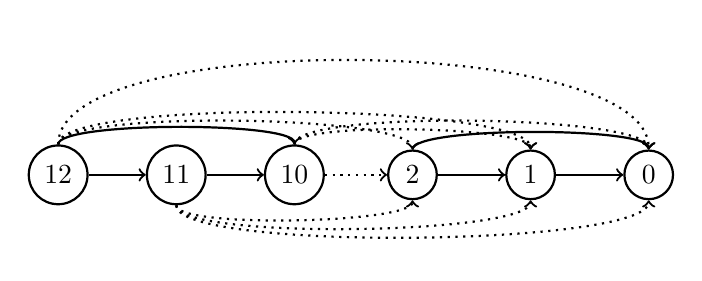
\begin{tikzpicture}[node distance={15mm}, thick, main/.style = {draw, circle}]
\node[main] (6) {$12$};
\node[main] (5) [right of=6] {$11$};
\node[main] (4) [right of=5] {$10$};

\node[main] (3) [right of=4] {$2$};
\node[main] (2) [right of=3] {$1$};
\node[main] (1) [right of=2] {$0$};
\draw[->] (6) -- (5);
\draw[->] (6) to [out = 90, in = 90, looseness=.25] (4);
\draw[->] (5) -- (4);

\draw[->] (3) -- (2);
\draw[->] (2) -- (1);
\draw[->] (3) to [out = 90, in = 90, looseness=.25] (1);

\draw[dotted][->] (6) to [out = 90, in = 90, looseness=.25] (3);
\draw[dotted][->] (6) to [out = 90, in = 90, looseness=.25] (2);
\draw[dotted][->] (6) to [out = 90, in = 90, looseness=.5] (1);

\draw[dotted][->] (5) to [out = 270, in = 270, looseness=.25] (3);
\draw[dotted][->] (5) to [out = 270, in = 270, looseness=.25] (2);
\draw[dotted] [->](5) to [out = 270, in = 270, looseness=.25] (1);

\draw[dotted][->](4) -- (3);
\draw[dotted][->](4) to [out = 90, in = 90, looseness=.25] (2);
\draw[dotted][->](4) to [out = 90, in = 90, looseness=.25] (1);

\end{tikzpicture}
\caption{Transitions between 6-die substates}
\label{fig:sixdietransitions}
\end{figure}


\begin{figure}[!htb]
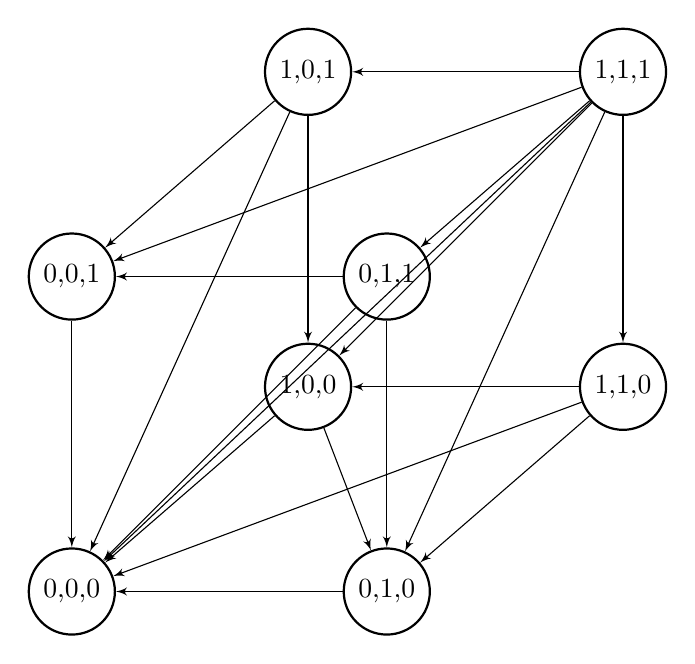
\begin{tikzpicture}
\begin{scope}[every node/.style={circle,thick,draw}]
\node (0) at (0, 0) {0,0,0};
\node (1) at (0, 4) {0,0,1};
\node (2) at (4, 0) {0,1,0};
\node (3) at (4, 4) {0,1,1};
\node (4) at (3, 2.6) {1,0,0};
\node (5) at (3, 6.6) {1,0,1};
\node (6) at (7, 2.6) {1,1,0};
\node (7) at (7, 6.6) {1,1,1};

\draw[edge] (1) to (0);
%\draw[edge] (2) to (1);
\draw[edge] (2) to (0);
\draw[edge] (3) to (0);
\draw[edge] (3) to (1);
\draw[edge] (3) to (2);
\draw[edge] (4) to (0);
%\draw[edge] (4) to (1);
\draw[edge] (4) to (2);
%\draw[edge] (4) to (3);
\draw[edge] (5) to (0);
\draw[edge] (5) to (1);
%\draw[edge] (5) to (2);
%\draw[edge] (5) to (3);
\draw[edge] (5) to (4);
\draw[edge] (6) to (0);
%\draw[edge] (6) to (1);
\draw[edge] (6) to (2);
%\draw[edge] (6) to (3);
\draw[edge] (6) to (4);
%\draw[edge] (6) to (5);
\draw[edge] (7) to (0);
\draw[edge] (7) to (1);
\draw[edge] (7) to (2);
\draw[edge] (7) to (3);
\draw[edge] (7) to (4);
\draw[edge] (7) to (5);
\draw[edge] (7) to (6);

\end{scope}
\end{tikzpicture}
\caption{Transitions between (B,C,D) = (8,10,12) substates}
\label{fig:cube}
\end{figure}


We can best visualize the transitions between these 104 states with the \emph{two} graphs in Figs.~\ref{fig:sixdietransitions} and ~\ref{fig:cube}.  The total state is exactly the combination of having anywhere from 0 to 12 6-dice left (Fig.~\ref{fig:sixdietransitions}) and having 0 or 1 (8-, 10-, 12-) dice left (Fig.~\ref{fig:cube}).  To conceptualize the whole graph in one figure, imagine breaking each of the $[0,1] \times 3$ nodes into a graph like (Fig.~\ref{fig:sixdietransitions}), and further, that every combined node $S_a = (a_6, a_8, a_{10}, a_{12})$ has a directed edge to node $S_b = (b_6, b_8, b_{10}, b_{12})$ if and only if $a_6 \leq b_6, a_8 \leq b_8, a_{10} \leq b_{10}, a_{12} \leq b_{12}, S_a \neq S_b$.

Given a state $S$ and the rolls we've gotten, we still want to choose to pick up the dice that give us the best expected value going forward.  This means running this algorithm to determine the expected value of state $S$:

\fbox{\parbox{\textwidth}{

\textbf{Pre-compute Algorithm: Expected value of die state $S$}:

\begin{enumerate}
\item Start with accumulator $z = 0$.
\item For each possible combination $c$ of rolls of $S = (a_6, a_8, a_{10}, a_{12})$ dice of size 6,8,10,12 respectively:
  \begin{enumerate}
    \item For each non-empty member $r$ of the power set $2^c$, where we take points and remove those $r$ dice:
    \begin{enumerate}
       \item Compute points added $P(r, c)$.
       \item Determine future state $S_+ = S_a - r$.
       \item Look up saved expected value $E_{S_+}$ from previous computations.
       \item Compute total value $E_{S}(r,c) = P(r, c) + E_{S_+}$ 
    \end{enumerate}
    \item Choose the $r^*$ with the highest value $E_{S}(r^*,c)$.
    \item Add $\frac{E_{s}(r^*, c)}{p(c)}$ to $z$, where $p(c)$ is the probability of combination $c$.
  \end{enumerate}
 \item Store $E_{s} \leftarrow z$.
\end{enumerate}
}}

We can precompute each such $E_{S}, S \in ([0,12 ] \times [0,1]^3 \in \mathbb{N}^4)$, in a \emph{reverse topological sort}, meaning crawling the graphs of Figs.~\ref{fig:sixdietransitions} and ~\ref{fig:cube} \emph{upstream} against the arrows, so that all of their required $E_{S_+}$ are ready for them.  An order might be doing all states with 0 dice, then 1 die, then 2 dice, like so:
\begin{itemize}
\item $S = (0,0,0,0)$ (known to be 0)
\item $S = (0,0,0,1)$ (known to be 6.5)
\item $S = (0,0,1,0)$ (known to be 5.5)
\item $S = (0,1,0,0)$ (known to be 4.5)
\item $S = (1,0,0,0)$ (known to be 3.5)
\item $S = (2,0,0,0)$
\item $S = (1,1,0,0)$
\item $S = (1,0,1,0)$
\item $S = (1,0,0,1)$
\item $S = (0,1,0,1)$
\item ...
\item $S= (3, 0, 0, 0)$
\item ...
\item $S = (12, 1,  1, 1)$
\end{itemize}

Finally, once all the $E_S$ are computed, in order to make the best choice during game time, the most straightforward correct algorithm is likely \emph{running steps (2a) and (2b) from the Pre-Compute algorithm above.}

This idea is an example of \emph{dynamic programming}, the idea of starting with less-complicated computations and saving the results to build to more complicated ones.  If we can rely on the previous computations as producing the best expected value, starting from known answers (the value of the empty state (0); the expected value of rolling a single die (3.5, 4.5, 5.5, 6.5 for our sizes)), the principle of choosing the move with the best expected value will produce, by extension, the best expected value at any larger state (including the 15-die state at the beginning of b.a.d.g.). 

\emph{Doing the pre-computation would be doable, but a pain.  Computing the truly best move in real-time would be a lot for a computer, and certainly impossible for a human.}.

\subsection{Why so difficult?}

Let's look at the volume of each of these steps in the \textbf{Algorithm} above to see the volume of these computations.
\begin{itemize}
\item Step 2.  \emph{... each possible combination $c$ of rolls of $S = (a_6, a_8, a_{10}, a_{12})$ dice of size 6,8,10,12 respectively:}

  \begin{itemize}
  \item At the beginning state, naively, with 12 six-sided dice, there are $6^12 = 2,176,782,336$ possible rolls if the dice are all, say, different colors.
  \item Noting that rolling $(1,1,2,2,3,3,4,4,5,5,6,6), (6,6,5,5,4,4,3,3,2,2,1,1)$ and $(1,6,1,6,2,5,2,5,3,4,3,4) $ are all the same, we can compute using the formula for ``12 indistinct balls in 6 distinct bins``\footnote{${12 + 6 - 1 \choose 6 - 1}$} to get 6188 truly different rolls.
  \item Combined with the possibilities for the other dice, this makes $(6188)(8)(10)(12) = 5,940,480$ rolls to consider at the beginning. 
  \item Naturally this is the biggest number of these. There may be only 6 rolls to consider at the end, perhaps.  Even in the middle (say, 6 6-sided dice, one 8-sided, one 10-sided), we're looking at 36,960 rolls.
  \end{itemize}
  
    
\item Step 2a: \emph{... each non-empty member $r$ of the power set $2^c$, where we take points and remove those $r$ dice}
  \begin{itemize}
  \item If there are 15 dice, the power set of these (minus the empty set\footnote{Gotta take at least one die!}) has $2^{15} - 1 = 32,767$ members.
  \item Again, looking in the middle of the game, $2^8 - 1 = 255$	 is still a lot to go through.
  \item We could mitigate this by not examining any choices  of $r$ where we accept multiple low-valued dice (half the pip count or less), which is never a good choice.  If half the values are low, then we're still left with examining something like $2^7=128$ possibilities.  Of course, we have to account for getting all ones in our expected value computation!
  \end{itemize}
\item The other computations are either simple (e.g. $p(c)$ in 2c) or already done ($E_S$ for an earlier state $S$).
\item And, of course, we need to do this 103 times\footnote{Empty set is a freebie: 0}, walking backward through the graphs in Figs.~\ref{fig:sixdietransitions} and ~\ref{fig:cube}.
\item If we took the average computation as the one where there are 6 6-sided dice, one 8-sided, and one 10-sided, that still totals $36960*255*103 = 970,754,400$ steps.  Of course, the middle is more like 7\% as hard as the beginning, not 50\%!
\end{itemize}

In the most optimistic case, we can pre-compute the value of all 104 expected states.  Then, for each of them we can generate a lookup table for the up to 6 million rolls possible.  Again, we can perhaps cut out some of the space where the die are high enough ($s$) or low enough ($\leq \frac{s}{2}$) for the answer to be obvious, but even specifying this strategy fully will take a lot of data.  

\textbf{It is possible that there is a perfect and compressible heuristic with a lot less data. We present an extremely small heuristic that should perform pretty well.}

\section{Splitting into parallel games} \label{section:split-out}

The main thesis of this paper: \textbf{We can reduce the game by considering 15 dice as each playing separate one-die games and bear the cost when this ends up being untrue.}  This produces a game with a compressible, human-scale strategy table, and a pretty good score (we think).

The value of this should be clear.  If we have N dice remaining, and each die is playing a one-die game with up to \emph{about} N possible rolls in its future, by the ``Know When to Quit'' principle, we should continue to roll that die until it's time to quit.

If this is the case, then our EV is clear from the lower-right entries in Figs.~\ref{fig:optimal6}, ~\ref{fig:optimal8}, ~\ref{fig:optimal10}, and ~\ref{fig:optimal12}.  12 6-dice with an EV best face of 5.859 (.141 points),, an 8-die with 7.762 (.328 points), a 10-die with 9.461 (.539 points), and a 12-die with 11.252 (.748 points), end up giving us an \textbf{expectation of 3.307 b.a.d.g. points.}.

However, this is not the case for two reasons:
\begin{itemize}
\item If we get lucky and start bagging lots of high rolls, we have fewer rolls ahead of us as we might ``skip'' from, say 15 dice left\footnote{15 dice means maximum 15 rolls} to 12 by picking up 3 instead of 1.  This is \emph{simultaneous fortune}.
\item If we get unlucky, we will be forced to choose pick up a die at or below its cutoff.  This is the main issue we'll face, or \emph{simultaneous misfortune}.  Within this:
  \begin{itemize}
  \item How often will we encounter misfortune?
  \item How much is it gonna cost us when do we?
  \end{itemize}
\end{itemize}

It's clear that we cannot declare that our strategy is the best \emph{only if nothing goes wrong}; just imagine we said ``Only pick up a die if it's the maximum.  If nothing goes wrong, your total score will be zero''.

But we'll focus on approximating the amount of pain we'll endure with this strategy, on top of the 3.307 points.  In particular, we'll focus on approximating the contribution of \emph{simultaneous misfortune}.

\emph{Simultaneous fortune} at least has two countervailing factors which may help cancel it out.  Simultaneously rolling a bunch of max rolls, say, helps us get a better score; it is clear we should always pick them up.  At the same time, it reduces the number of at-bats for the other dice by a little bit.   For a game of 12 6-sided dice, rolling three sixes betters our expected b.a.d.g. score for those dice by (.243 * 3 = .729) points, while the other nine see their expected score rise to .42 from .291 (1.161 points).  On the other \emph{other} hand, big jumps make the game shorter, and a shorter game has a smaller chance of the misfortune that actually does damage to us (makes us eat points), \emph{simultaneous misfortune}.  In reality, simultaneous fortune is an unalloyed good.  The only way it ``hurts us'' is merely accounting: it simply makes the remainig dice's expected values derived from  the ``separate games''  simplification less accurate.

Each b.a.d.g. game is a walk through the 104-node graph of Figs.~\ref{fig:sixdietransitions} and ~\ref{fig:cube}, taking between one and fifteen steps.  The number of such paths bears a lot of similarity to the large numbers of the previous section.  

Let's just look at a typical `seeming' path to get a sense of our chance of simultaneous fortune and misfortune, with a maximum likelihood estimate at each step.

The chance of simultaneous misfortune for a set of dice $S=(a,b,c,d)$, with cutoffs $(c_a, c_b, c_c, c_d)$ is $P_m(a,b,c,d) = (\frac{c_a}{6})^a (\frac{c_b}{8})^b (\frac{c_c}{10})^c (\frac{c_d}{12})^d$.  Using the tables for our strategy, let's take a typical seeming walk.
\begin{comment}
\begin{itemize}
\item 15 dice.  $S = (12, 1, 1, 1).  P_m(S) = (5/6)^{12}*7/8*9/10*11/12 = 0.081.$  &  $(2, 0.125, 0.1, 0.083)$
\item 13 dice. $S = (10, 1, 1, 1). P_m(S) = (5/6)^{10}*7/8*9/10*11/12 = 0.117$.  &  $(3.67, 0.25, 0.2, 0.166)$
\item 11 dice. $S =  (8,1,1,1).  P_m(S) = (5/6)^8*7/8*9/10*10/12  = 0.153$.  &  $(5, .375, .3, .25)$
\item 10 dice. $S= (7,1,1,1).  P_m(S) = (5/6)^7*7/8*8/10*10/12 = .163$.  &  $(6.17, .5, .4, .33)$.  Take off at .5.
\item 8 dice. $S= (6,0,1,1).  P_m(S) = (5/6)^6*8/10*10/12 = .223.$.  &  $(7.17, .625, .5, .42)$.  Keep on at .5.
\item 7 dice. $S= (5, 0, 1, 1).   P_m(S) = (5/6)^5*8/10*10/12 = .268$.  &  $(8, .75, .6, .5)$.  Take off at .5.
\item 4 dice. $S= (4,0,0,0)   P_m(S) = (4/6)^4 = .198.$  &  $(8.66, ...)$
\item 3 dice. $S= (3,0,0,0)   P_m(S) = (4/6)^3 = .297.$  &  $(9.16, ...)$
\item 2 dice. $S= (2,0,0,0)   P_m(S) = (3/6)^2 = .25.$  &  $(9.5, ...)$
\item 1 die. $S= (1,0,0,0) $.  There is no misfortune here.  
\end{itemize}
\end{comment}




\begin{figure}[!htb]
\centering
\begin{tabular}{c | c c c}
dice & State & $P_m(S)$  & Exp hits \\
\hline
15 & $(12, 1, 1, 1).  $ & $ (5/6)^{12}*7/8*9/10*11/12 = 0.081.$  & $(2, 0.125, 0.1, 0.083)$\\
13 & $(10, 1, 1, 1)$ &  $  (5/6)^{10}*7/8*9/10*11/12 = 0.117$.  &  $(3.67, 0.25, 0.2, 0.166)$\\
11  & $(8,1,1,1)$ & $(5/6)^8*7/8*9/10*10/12  = 0.153$.  &  $(5, .375, .3, .25)$ \\
10  & $(7,1,1,1)$ & $(5/6)^7*7/8*8/10*10/12 = .163$.  &  $(6.17, .5, .4, .33)$.   \\
8  & $(6,0,1,1)$ & $(5/6)^6*8/10*10/12 = .223.$.  &  $(7.17, .625, .5, .42)$.  \\ 
7  & $(5, 0, 1, 1)$ &   $(5/6)^5*8/10*10/12 = .268$.  &  $(8, .75, .6, .5)$.   \\ 
4  & $(4,0,0,0)$   & $4/6)^4 = .198.$  &  $(8.66, ...)$ \\
3  & $(3,0,0,0)$   &$(4/6)^3 = .297.$  &  $(9.16, ...)$ \\ 
2  & $(2,0,0,0)$  &$(3/6)^2 = .25.$  &  $(9.5, ...)$\\ 
1 & $(1,0,0,0)$ & 0 & \\
\end{tabular}
\caption{A random walk down Waldman St.}
\label{fig:walk}
\end{figure}


We have, for this walk, an expected 1.75 occurrences of simultaneous misfortune.  Let's estimate that we only lift one die\footnote{Though \emph{maybe} if two dice are very close to their EV, there's a corner case where lifting two is correct} and we pay a cost of between 1 (almost certain for early misses) and 2 (a bad final roll won't, on average penalize us all that much either), so a hand-wavy contribution of 1.5, for a total of 1.5*1.75=2.625 extra b.a.d.g. points on top of our 3.307 for 5.932.  

There is no simple way to denote this a truly average walk.    The only reasonable way to evaluate either with any accuracy is just simulation with our strategy.  

\section{Simulation} \label {section:simulation}

\begin{comment}
\begin{lstlisting}
import random

# Tables
six_cutoffs = [ -1, -1, 3, 4, 4, 4, 5, 5, 5, 5, 5, 5, 5, 5, 5, 5]
eight_cutoffs = [ -1, -1, 4, 5, 6, 6, 6, 6, 7, 7, 7, 7, 7, 7, 7, 7]
ten_cutoffs = [-1, -1, 5, 6, 7, 7, 8, 8, 8, 8, 8, 9, 9, 9, 9, 9]
twelve_cutoffs = [ -1, -1, 6, 7, 8, 9, 9, 10, 10, 10, 10, 10, 10, 11, 11, 11]

initial_die_state = [12, 1, 1, 1]

def argmin(l):
    index, min_val = -1, 1000
    for i in range(len(l)):
        if l[i] < min_val:
            index, min_val = i, l[i]
    return index

def trymax(l):
    if (len(l) == 0):
        return -100000
    else:
        return max(l)
    
def generate_rolls(die_state, verbose=False):
    dice_left = sum(die_state)
    rolls = [[random.randint(1,6) for i in range(1,die_state[0] + 1)],
              [random.randint(1,8) for i in range(1,die_state[1] + 1)],
              [random.randint(1,10) for i in range(1,die_state[2] + 1)],
              [random.randint(1,12) for i in range(1,die_state[3] + 1)]]
    
    verbose and print(rolls)

    good_rolls = [ list(filter(lambda x: x > six_cutoffs[dice_left], rolls[0])),
                   list(filter(lambda x: x > eight_cutoffs[dice_left], rolls[1])),
                   list(filter(lambda x: x > ten_cutoffs[dice_left], rolls[2])),
                   list(filter(lambda x: x > twelve_cutoffs[dice_left], rolls[3]))]

    verbose and print(good_rolls)
    if (good_rolls != [[], [], [], []]):
        six_points = 6 * len(good_rolls[0])  - sum(good_rolls[0])
        six_removed = len(good_rolls[0])

        eight_points = 8 * len(good_rolls[1])  - sum(good_rolls[1])
        eight_removed = len(good_rolls[1])

        ten_points = 10 * len(good_rolls[2])  - sum(good_rolls[2])
        ten_removed = len(good_rolls[2])

        twelve_points = 12 * len(good_rolls[3])  - sum(good_rolls[3])
        twelve_removed = len(good_rolls[3])

        points = six_points + eight_points + ten_points + twelve_points
        die_state = [die_state[0] - six_removed, die_state[1] - eight_removed, die_state[2] - ten_removed, die_state[3] - twelve_removed]

        return [points, die_state, 0]
    else:
        # -100 is a bad hack to give a max on an empty set
        best_rolls = [six_cutoffs[dice_left] - trymax(rolls[0]) , 
                      eight_cutoffs[dice_left] - trymax(rolls[1]),
                      ten_cutoffs[dice_left] - trymax(rolls[2]), 
                      twelve_cutoffs[dice_left] - trymax(rolls[3])]
        verbose and print ("Best rolls")
        verbose and print(best_rolls)
        removable_die_pos = argmin(best_rolls)
        points = [6,8,10,12][removable_die_pos] - trymax(rolls[removable_die_pos])
        
        die_state[removable_die_pos] = die_state[removable_die_pos] - 1

        verbose and print("Removing die at pos %s " % (removable_die_pos))
        return [points, die_state, 1]

    
def run_sim():
    die_state = [12, 1, 1, 1]
    points = 0
    interruptions = 0
    while die_state != [0, 0, 0, 0]:
        result_vec = generate_rolls(die_state, verbose=False)
        points = points + result_vec[0]
        die_state = result_vec[1]
        interruptions = interruptions + result_vec[2]
    return [points, interruptions]

def averages(v):
    return [
        sum(list(map(lambda x: x[0], v))) / len(v),
        sum(list(map(lambda x: x[1], v))) / len(v)]

     

\end[lstlisting}
\end{comment}

\end{document}
